\documentclass[conference, 10pt]{IEEEtran}
\usepackage{graphicx}
\usepackage{enumerate}
\usepackage{amsmath}
\usepackage{xspace}
\usepackage{cite}
\usepackage[linesnumbered]{algorithm2e}
\usepackage{subfig}
\usepackage{minted}
\usepackage{textcomp}
\usepackage{hyperref}

\newcommand*{\eg}{e.g.\@\xspace}
\newcommand*{\ie}{i.e.\@\xspace}

\makeatletter
\newcommand*{\etc}{%
    \@ifnextchar{.}%
        {etc}%
        {etc.\@\xspace}%
}
\makeatother

\begin{document}

\title{CS270 Course Project Report:\\
Quick Alignment Algorithm for Burst Photography}

\author{\IEEEauthorblockN{Rundong Li}
\IEEEauthorblockA{36273800\\
SIST, ShanghaiTech University}
}

\maketitle

\begin{abstract}
    Photography quality of cell phones has received lot of attention. 
    Limited by small radius lens and tiny COMS sensors, digital images captured by
    mobile phones are easily suffer from noise on low illuminated areas, and unable to capture
    dynamic range on strongly illuminated areas. One possible solution is taking a burst of frames with different
    exposure settings, then merging into single high quality image.
    This rises the challenge of effectively aligning different frames before or after a series
    of other sophisticated operations. 
    We try to address this challenge in this course project.

    Note: to meet the strict constrains of real-world applications, the proposed algorithm
    is quite straight forward but implementing it requires lots of engineering efforts.
    Thus we organize this report more like a technical manual than academic paper, 
    focusing on the engineering decisions and optimization techniques we taken, as well as the algorithm itself.
\end{abstract}

\section{Scope}

This technical manual describes the design, implementation and optimization of L1/L2 mixed
alignment algorithm based on \cite{hasinoff2016burst}. This manual is organized as following sections:
\begin{enumerate}
    \item Proposed algorithm and application scenario;
    \item Implementation and optimization;
    \item Results and discussions;
\end{enumerate}

This implementation is open-sourced at \url{https://github.com/CrazyRundong/burst-align} under GPL-v3 License.

% ==============================================================================
\section{Proposed Algorithm and Application Scenario}

One possible technique to address dark noise and poor dynamic range introduced by
optical and semiconductor limitations are generating HDR pictures by burst photography \cite{kayvon18visual, liu2014fast}.
To be brief, burst photography means taking several frames with different exposure settings
within certain time window, pick one sharpest frame as \emph{reference frame},
then merge corresponding regions among remaining \emph{alternative frames} to
perform denosing and dynamic range adjustment (Figure \ref{img::intro}). One key challenge is to locate and
match these corresponding regions. This locate-and-match procedure is called \emph{alignment}.

Precision-targeted alignment problem is well-studied, solutions include optical flow \cite{horn1981determining},
dense corresponding \cite{liu2011sift}, and over-segmentation then directly reason about geometry and occlusion
\cite{yamaguchi2014efficient}. In order to acquire high alignment precision, these solutions are usually slow and computation expensive,
\eg the top-5 entries on KITTI optical flow benchmark \cite{menze2015object} require between
1.7 to 107 minutes to perform complete alignments per M-pixes.

However, majority of application scenarios of burst photography are relevant to mobile devices, \eg
cell phones and drones with small radius lens and tiny COMS sensors. Computation budgets of these
devices are quite constrained, alignment algorithms thus should be efficient and fast.
We propose a tile-based, coarse to fine alignment algorithm, named \emph{L1/L2 mixed alignment}
based on fast L2 alignment proposed in \cite{hasinoff2016burst} and fast cross-correlation
proposed in \cite{yoo2009fast}.

\begin{figure}[tb]
\centering
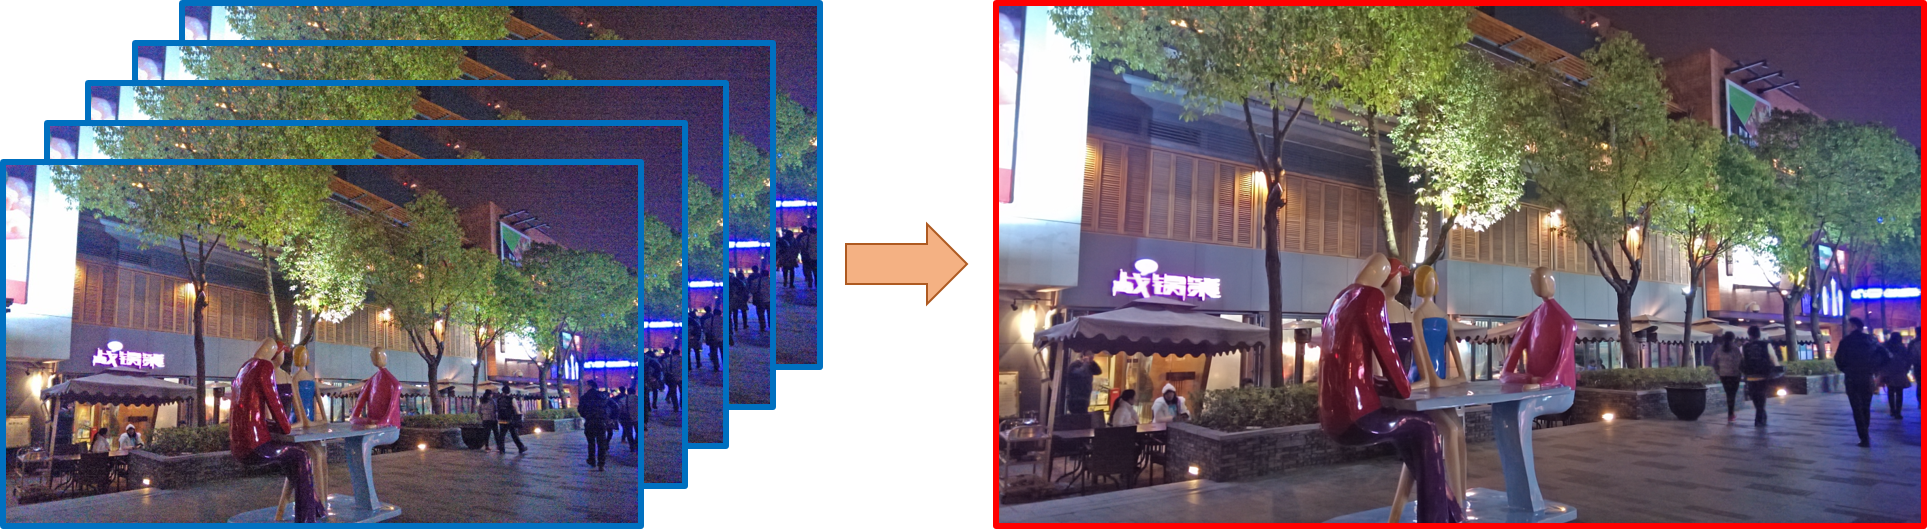
\includegraphics[width=\columnwidth]{img/intro_Liu_SIGGRAPH14.png}
\caption{A burst of frames can be align and merged into single high dynamic range photo. \cite{liu2014fast}}
\label{img::intro}
\end{figure}

The proposed L1/L2 mixed alignment algorithm is quite straight forward: we firstly split
reference frame into \emph{regions}, then search corresponding regions on alternative
frames. Once a certain region in an alternative frame is find to match the reference region,
the output alignment of this pair of regions is set to their spatial mismatches.

Detailed design decisions of proposed algorithm include:

\paragraph{Corresponding regions are rectangle tiles} Instead of performing pixel-wise
alignment, our minimum alignment units are rectangle regions called \emph{tiles}.
This decision is based on: objects are not likely to have obvious deformation within short time
window, rectangle tiles thus can be served as good matching template;

\paragraph{Restricting search regions and introducing image pyramids to reduce computation}
Search regions should be large enough to capture moving object among frames, however computation
costs is squared w.r.t. search region size. Thus we firstly scale input frames into different
spatial sizes, computing alignment on coarsest frames, then search matching tiles on
larger frames starting from interpolated previous alignments. Search regions can be restricted
thanks to this interpolate and initializing strategy;

\paragraph{Tile matchness on coarse levels are measured by L2 distance...} 
As illustrated in \S 4.1 of \cite{hasinoff2016burst}, computing
L2 distances among one fixed tile (T) and a slide tile (I) within a search region can be implemented
as one un-normalized box-filter plus a FFT-based matrix multiplication:
\begin{align*}
    D_2(u, v) &= \sum_{y=0}^{n-1} \sum_{x=0}^{n-1} \| T(x, y) - I(x + u + u_0, y + v + v_0) \|_2^2 \\
              &= \| T \|_2^2 + \mathrm{box}(I \circ I, n) - 2\mathcal{F}^{-1}(\mathcal{F}(I) \circ \mathcal{F}(T))
\end{align*}
where $D_2$ is the L2 distance between reference tile at $(u, v)$ and alternative tile at $(u + u_0, v + v_0)$,
$T$ is the reference frame, $I$ is current alternative frame, $n$ the size of tile,
and $(u_0, v_0)$ the interpolated alignment (the ``start point'') from coarser pyramid level.

\paragraph{...and use L1 distance on largest pyramid level} Although L2 distance
computation can be optimized in algorithm level, on largest search size the brute force
L1 distance computation is still faster than optimized L2 implementation. \eg on
\texttt{x86\_64} platform, absolute value computing can be accreted by \texttt{\_mm\_abs\_pi8}
intrinsic \cite{Intel2015abs}.

After all, the proposed L1/L2 mixed alignment can be formulated as Algorithm \ref{algo::mix_align}.
Next we describe the details in our implementation and optimization.

\begin{algorithm}[tb]
    \KwData{reference frame $I_{ref}$, alternative frames $I_{1\ldots N}$, image pyramid level $L$,
    downsample ratio $r_{1 \ldots L}$ at each pyramid level,
    tile size $t_{1 \ldots L}$ at each pyramid level, search region $s_{1 \ldots L}$ at each pyramid level;}
    \KwResult{alignment map $D_{1 \ldots N}$ on each alternative frames w.r.t. $I_{ref}$;}

    \BlankLine
    % \tcp{prepare image pyramid for $I_{ref}$}
    $P_{ref} = \emptyset$\;
    \For{$r \leftarrow r_{1 \ldots L}$}{
        $P_{ref} = P_{ref} \cup \{ \mathtt{avg\_pool}(I_{ref}, r) \}$\;
    }

    \For{$n \leftarrow 1\ldots N$}{
        $P_{alt} = \emptyset$\;
        \For{$r \leftarrow r_{1 \ldots L}$}{
            $P_{alt} = P_{alt} \cup \{ \mathtt{avg\_pool}(I_n, r) \}$\;
        }
        \For{$i \leftarrow L\ldots 1$}{
            % \tcp{compute number of tiles on level $i$}
            $n_H = P_{ref}[i].height / \frac{t_i}{2} - 1$\;
            $n_W = P_{ref}[i].width / \frac{t_i}{2} - 1$\;
            \eIf{$i == L$}{
                $d_{i} = \mathtt{zeros}(n_H, n_W, 2)$\;
            }{
                $d_{i} = \mathtt{interpolate}(d_{i+1}, n_H, n_W)$\;

            }
            split $P_{ref}[i]$ and $P_{alt}[i]$ into tiles $T_{ref}$ and $T_{alt}$\;
            \For{$y \leftarrow 1 \ldots n_H$}{
                \For{$x \leftarrow 1 \ldots n_W$}{
                    \For{$dx, dy \in s_i$}{
                        \eIf{i == 1}{
                            use L1 distance $dist_1$\;
                        }{
                            use L2 distance $dist_2$\;
                        }
                        $a_y, a_x = \arg_{dx, dy}\, \min \,dist(T_{ref}[y, x],
                                    T_{alt}[y + dy + d_i[y, x, 0],
                                    x + dx + d_i[y, x, 1]])$\;
                        $d_i[y, x, 0] = a_y$\;
                        $d_i[y, x, 1] = a_x$\;
                    }
                }
            }
            \If{$i == 1$}{
                $D_n = d_i$\;
            }
        }
    }
\caption{Tile based L1/L2 mixed alignment.}
\label{algo::mix_align}
\end{algorithm}

% ==============================================================================
\section{Analysis, Implementation and Optimization} \label{sec::imp}

For demonstrating purpose, we firstly build a pure Python implementation 
\href{https://github.com/CrazyRundong/burst-align/blob/master/demo.py}{\texttt{demo.py}}.
As will be illustrated in \S \ref{sec::exp}, this algorithm can yield reasonable results
but the naive loop-based Implementation requires $\sim 127$ seconds for each burst,
which is infeasible for real-world deployment.

To speed up this implementation, we firstly analysis Algorithm \ref{algo::mix_align}, try to
identify potential optimization opportunities. Next we implement these optimizations by generated
C-language kernels and evaluate the performance gain. Finally we explain other engineering details
and efforts we had taken to ensure the correctness and precision of our implementation.

% ------------------------------------------------------------------------------
\subsection{Analyze the Algorithm} \label{sec::analyze}

The proposed L1/L2 mixed alignment is basically a brute-force search with inherent
parallelism, we analysis this algorithm along the formulation in 
Algorithm \ref{algo::mix_align} to identify optimization opportunities.

\paragraph{For alternativa frames} This out-most loop (line 5 to 37) is both data and control independent
among each loop steps. However parallelize in this granularity could be unfriendly
to memory: note that memory location of each alternative images $I_{1 \ldots N}$
could be different, memory accessing continuity thus could not be guaranteed if we
spawn a pool of threads and let each thread align one of the alternative images.

\paragraph{For pyramid levels} To restrict the search region size, each search step is initialized by
interpolated previous search steps (line 10 to 36, the initializing
logic is from line 13 to 17). Because of this data-dependency, parallelism can not
be applied along each pyramid levels. However, there still exist optimization opportunities
on initializing step: note the interpolate operation in line 16 and pooling operation in
line 8. Since these operations are nearly element-wised and is performed on continuous
$I_n$ and $d_{i+1}$, we could parallel along the rows of these operations before
optimizing the next-step alignments.

\paragraph{For search tiles} \label{sec::for_tile} Tile-based searching is formulated as double-loop (line 19
to line 32). The number of tiles spans from $6$ (the top-most pyramid level) to $\sim 188$K
(the bottom pyramid level) for 13M-pixes input, the search process and output location
of each tiles are not conflict to others. Thus we can easily get speedup by launching
multiple threads, each thread for aligning one tile.
Note that a large number of threads will be launched on lower pyramid levels,
if all these threads executed in parallel, memory bandwidth could immediately
become performance bottleneck.
However the deploy target, ARM or x86\_64 CPU, is usually capable of executing only
$4 \sim 16$ threads in parallel, so we shall not take too much concern about the memory
bandwidth problem.

\paragraph{For search locations} \label{sec::simd} Each tile will slide though a rectangle search region
(line 19, 20) and accumulate pixel wise differences. Since we have assigned all threads
to each tiles as described in previous paragraph, no further parallelism could be utilized.
However, since most of modern CPUs do support single-instruction-multiple-data (SIMD) execution
pattern, we can further vectorize the subtraction and accumulation procedure on each
search location, then utilize SIMD intrinsic to get more speedups.

SIMD basically means that, target CPU gets multiple arithmetic logic units (ALUs)
available at each pipeline step, so multiple data could be loaded, computed and
dumped at single instruction time. These instructions are wrapped as hardware-specific,
language-level \emph{intrinsics} so we could not be bothered writing assemble to
get SIMD speedup. 
\eg when computing the L1 distances between two 32-element 16-bit ({\tt unsigned short} for C99) row-vector 
$I_{0\ldots 31}$ and $T_{0\ldots 31}$, instead of performing 32 loop steps
\begin{minted}{c}
T tmp = 0;
for (int i = 0; i < 31; ++i) {
    tmp += fabs(I[i] - T[i]);
}
\end{minted}
we can use {\tt \_mm512\_sub\_epi16} intrinsic to do these 32 subtractions, then use {\tt \_mm512\_add\_epi16} to accumulate all
32 elements, both in \emph{single instruction time}:
\begin{minted}{c}
__mm512i i_vec = _mm512_loadu_epi16(I);
__mm512i t_vec = _mm512_loadu_epi16(T);
__mm512i dst;
dst = _mm512_sub_epi16(i_vec, t_vec);
dst = _mm512_abs_epi16(dst);
// take reduction sum
dst = _mm512_add_epi16(dst,
      _mm512_srli_epi16(dst, 16));
\end{minted}
As illustrated above, the computation heavy logic could be optimized from $> 32$ instruction
time to $3$ instruction time.

% ------------------------------------------------------------------------------
\subsection{Optimizations}
In this section we describe the implementation of aforementioned optimizations.

\paragraph{Rewrite performance-critical code by C} As illustrated in Algorithm \ref{algo::mix_align},
vast majority of alignment precess is based on loop, which is difficult to vectoring.
Besides the analysis we investigated in \S \ref{sec::analyze},
we run Python performance profiler \href{https://docs.python.org/3.7/library/profile.html}{\texttt{cProfile}}
to locate the performance-critical code, then rewrite them by C-language kernels.
To be specific, we rewrote the average pooling kernels, the bilinear interpolate kernels
and per-layer alignment kernels (line $18 \sim 32$ in Algorithm \ref{algo::mix_align})
in \texttt{Cython} format then generate efficient C- code by \cite{behnel2011cython}.

\paragraph{Utilize parallelism} As we discussed in \S \ref{sec::analyze}, we decide
to parallel at three granularity: the element-wise down-sampling and interpolation,
and the dependency-free tile-wise searching. To be specific, for down-sampling and interpolation,
since the internal matrices, \eg input images and alignment maps, are all C-styled
row-major memory chunk, we thus apply OpenMP \cite{dagum1998openmp} on the row-level,
so each thread could be able to access continuous memory. OpenMP is wrapped into
{\tt prange} (paralleled range) in Cython:
\begin{minted}{Cython}
for i in prange(h_out, nogil=True):
    for j in range(w_out):
        # compute scaling and indexing...
        for c in range(channels):
            # per-channel weighted sum...
\end{minted}
Note that we have taken out the GIL (Global Interpreter Lock) \cite{Sajip2009GIL} in the
beginning of OpenMP invoking by {\tt nogil=True}. This is necessary for speedup
Cython generated C-code, otherwise the GIL will prevent multiple CPU cores from executing
spawned threads in parallel.

\paragraph{Utilize vectorization} As analysis in \ref{sec::simd}, when iterating $dx$ though
$T_{ref}, T_{alt}$, both cache and memory is continuous, thus we use Intel x86\_64
intrinsics to optimize the search loop (line 21 to 30). Since our experiment platform
is equipped AVX2-enabled Intel i7-8750H CPU \cite{Intel8750}, we used the intrinsic
{\tt \_mm512\_sub\_epi16, \_mm512\_abs\_epi16} and {\tt \_mm512\_add\_epi16} available on AVX2 instruction set
to compute the L1 distance. These three intrinsics are used to compute vector subsection,
vector absolute value and vector accumulation, respectively.
The computation pattern is identical to our previous discussion.

All above optimizations can be find in our Cython implementation 
\href{https://github.com/CrazyRundong/burst-align/blob/master/align/align_cpu.pyx}{\texttt{align\_cpu.pyx}}.
As will be illustrated in \S \ref{sec::exp},
these optimizations introduce orders of magnitudes of accelerating to our implementation.

% ------------------------------------------------------------------------------
\subsection{Other Implementation Details}

There are several other implementation details in our optimization. We modified the
bilinear interpolate algorithm to get better interpolates on image corners. We also
write unit tests for all C-kernels to ensure the correctness.

\paragraph{Corners in bilinear interpolation} In standard bilinear interpolation, 
when computing the output value $y(u, v)$ from input $x$ and scale factor $s$, source indices
are usually taken by directly multiply output indices by scale factor, \eg:
\begin{align*}
    u_0 &= \lfloor u \cdot s \rfloor \\
    u_1 &= \lceil u \cdot s \rceil
\end{align*}
However, when interpolating four corner pixels, output values are sampled from only the relevant
source input, thus context information will be miss. We thus add a little ``bias''
to the source selection:
\begin{align*}
    u_0' &= \lfloor (u + 0.5) \cdot s - 0.5\rfloor \\
    u_1' &= \lceil (u + 0.5) \cdot s - 0.5\rceil
\end{align*}
Since 2d bilinear interpolations are all sampled from adjacent pixels, this little
``bias'' can help improve the quality of interpolation corners.

\paragraph{Unit tests for C-kernels} Since we must ensure the correctness of our
implementation before and after each optimization, we wrote unit tests for all C-kernels.
To be specific, we use {\tt pytest} framework to run coverage tests, test input are
random tensors generated by RNG with deterministic random seed, test ground truth
are generated by PyTorch {\tt nn.AvgPool2d, nn.BilinearUpsample2d} functions, alignment
ground truth is set to the naive Python alignment output. Detailed implementations
could be find at \href{https://github.com/CrazyRundong/burst-align/blob/master/test/test_align_cpu.py}{\tt test\_align\_cpu.py}.

% ==============================================================================
\section{Results and discussions} \label{sec::exp}

In this section we illustrate our experimental results on HDR+ dataset \cite{hasinoff2016burst}
and accelerating introduced from our optimizations.

\begin{figure}[tb]
\centering
\subfloat[alignment with 3-level image pyramid]{
    \label{img::align_3}
    \begin{minipage}{\columnwidth}
    \centering
    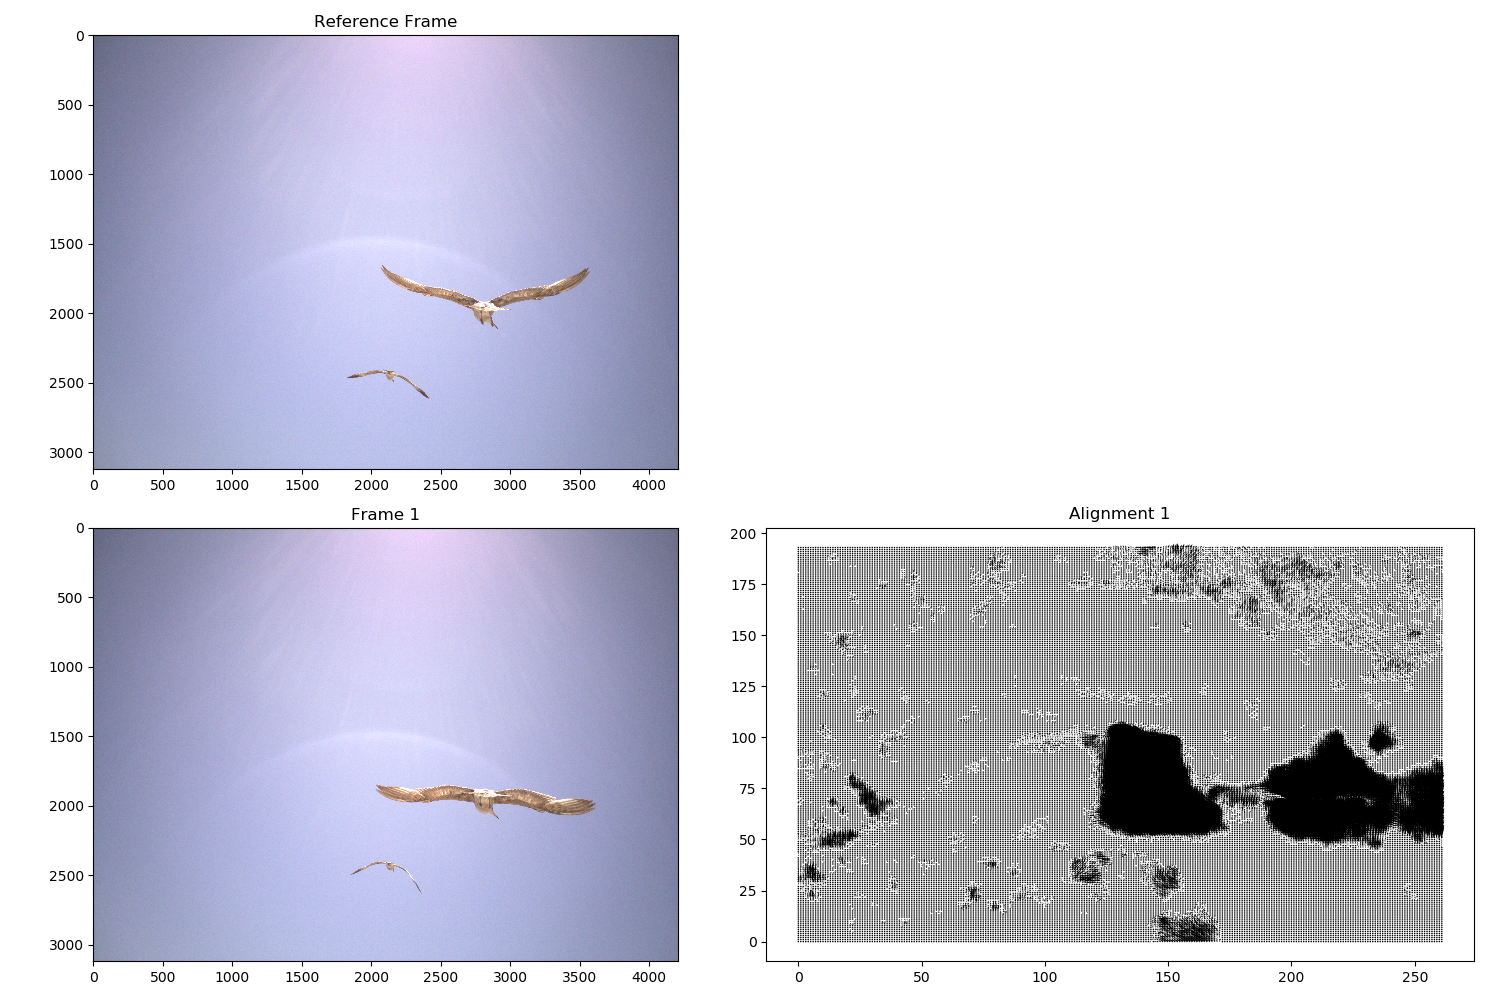
\includegraphics[width=\columnwidth]{img/demo_3_level.png}
    \end{minipage}
}
\newline
\subfloat[alignment with 4-level image pyramid]{
    \label{img::align_4}
    \begin{minipage}{\columnwidth}
    \centering
    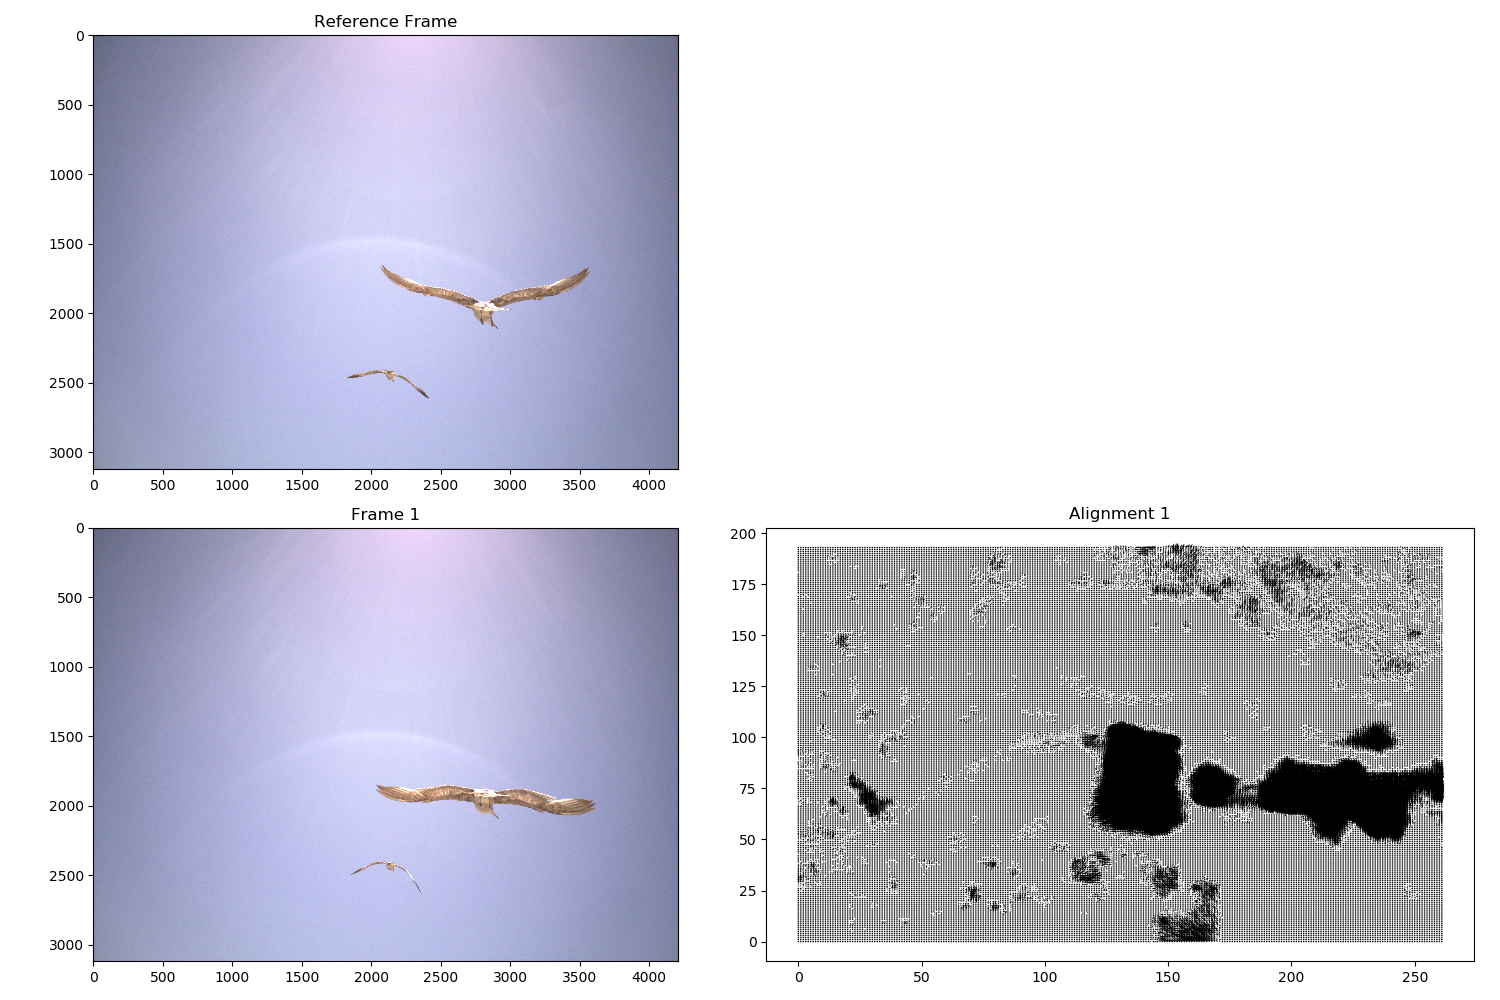
\includegraphics[width=\columnwidth]{img/demo_4_level.png}
    \end{minipage}
}
\caption{Alignment on burst with moving objects. In both sub-figures, top-left
is the reference frame, bottom-left is the alternative frame, right-bottom is the
alignment map.}
\label{img::aligns}
\end{figure}

In Figure \ref{img::aligns} we illustrate the results from proposed algorithm, applied
on a burst of seagull images taken from HDR+ dataset. In Figure \ref{img::align_3},
alignment map is computed by a 3-level image pyramid, while in Figure \ref{img::align_4}
a 4-level image pyramid is used. In both settings, each pyramid level is downsampled
by ratio of 4 from previous level, tile size on each pyramid level
is set to 16, search regions is within a $\pm 4$ pixes rectangle for each tile.

Proposed algorithm successfully matched corresponding regions on both settings
(see the response areas on alignment maps, which are wings of seagulls). Note that when
deeper pyramid is used (Figure \ref{img::align_4}), the alignment algorithm will
generate less false-positive responses (see the left-bottom regions of alignment
maps). However deeper pyramid requires more computation budget, so this accuracy-speed
tradeoff should be taken into consideration when applying this algorithm in real-world applications.

Another important criterion of proposed algorithm is speed. We benchmark our implementations
on a laptop with $2.2$GHz Core i7 processor.
As illustrated in Table \ref{tab::speed}, after utilizing the optimizations we proposed in
\S \ref{sec::imp}, time consumption
of aligning two 13M-pixes raw images reduces from $127.47$ seconds to $0.32$ seconds, which
gives us $\mathbf{398.34}\times$ speedup.
Also note that our implementations runs at $2.94$ FPS, which should be fast enough
for real-world applications. Further speedup can be archived by more aggressive
optimizations, \eg using OpenCL or CUDA to further utilize parallelism.

\begin{table}
    \begin{center}
    \small
    \begin{tabular}{r | ccc}
    \hline
    Implementation & Input & Pyramid level & Time \\
    \hline
    naive Python & 13M-pix $\times 2$ & 3 & 127.47s \\
    multi-thread C & 13M-pix $\times 2$ & 3 & \textbf{0.32}s \\
    multi-thread C & 13M-pix $\times 2$ & 4 & 0.35s \\
    multi-thread C & 13M-pix $\times 10$ & 3 & 3.40s \\
    \hline
    \end{tabular}
    \end{center}
\caption{Running time of our implementations.}
\label{tab::speed}
\end{table}

\bibliographystyle{IEEEtran}
\bibliography{report_ref.bib}

\end{document}
